\documentclass{beamer}

\usetheme{Madrid}
\setbeamertemplate{navigation symbols}{}
\setbeamertemplate{footline}[frame number]
\usepackage{graphicx}
\graphicspath{{figures/}}

\title{Hedging Against Turkish Inflation}
\author{Selin Acar, Necati Furkan Çolak, Denis Lasser}
\date{December 2024}

% Bibliography setup
\usepackage[round]{natbib}
\bibliographystyle{plainnat}
\setbeamertemplate{bibliography item}[text]

\begin{document}

% Title Page
\frame{\titlepage}

% Table of Contents
\begin{frame}{Outline}
\tableofcontents
\end{frame}

% Introduction I
\section{Introduction}
\begin{frame}{Introduction I}
\begin{itemize}
\item Ongoing economic crisis in Türkiye has been characterized by
\textbf{high inflation}, the \textbf{depreciation of the Turkish Lira}
(TRY), \textbf{rising borrowing costs}, and \textbf{increasing loan
defaults}.
\item The underlying causes of the crisis can be attributed to
\textbf{political instability}, \textbf{global economic pressures},
and the implementation of \textbf{unconventional economic policies}.
\item Since 2018, inflation has been a persistent issue, partly due to
fluctuations in global oil prices and exchange rates, with
\textbf{Turkey's inflation rate ranking among the highest in emerging
markets} \citep{yilmazkuday_2022}.
\end{itemize}
\end{frame}

% Introduction II
\begin{frame}{Introduction II}
\begin{itemize}
\item The Turkish government's policy of maintaining low interest rates to
stimulate growth, despite the conventional theory that raising
interest rates should reduce inflation, has contributed significantly
to the current economic challenges \citep{kantur_ozcan_2021}.
\item Interest rates have been raised significantly. The most recent rate
hike was in March 2024, when the central bank increased the
\textbf{interest rate} by 5 percentage points to \textbf{50\%} as the
year-on-year inflation reached 75\% \citep{bloomberg_2024}.
\item Since then, the rate has remained unchanged as the central bank has
been committed to fighting high inflation and stabilising the Turkish
lira. As of October 2024, \textbf{year-on-year inflation stands at
48\%} \citep{bloomberg_2024}.
\end{itemize}
\end{frame}

% Methodology I
\section{Methodology}
\subsection{Asset Performance Analysis}
\begin{frame}{Methodology: Asset Performance Analysis}
\begin{itemize}
\item Analyze asset performance using monthly data (Jan 2018--Sep 2024).
\item Two steps:
\begin{enumerate}
\item Evaluate individual asset hedging effectiveness.
\item Construct an optimal hedging portfolio using Markowitz optimization.
\end{enumerate}
\end{itemize}
\end{frame}

% Methodology II
\subsection{Data Sources}
\begin{frame}{Methodology: Data Sources}
\begin{itemize}
\item From Bloomberg:
\begin{itemize}
\item \textbf{TUCXEFYY Index}: Turkish core CPI (excluding food, energy,
alcohol, tobacco).
\item \textbf{XU100 Index}: Turkish stock index (BIST 100).
\item \textbf{GTTRY10YR}: 10-Year Turkish Government Bond.
\item \textbf{XAU}: Global prices in USD. 
\item \textbf{XBT BGN}: Bitcoin prices in USD.
\item \textbf{USGG10YR Index}: 10-year US Government Bond Yield as the risk free rate.
\end{itemize}
\item From Turkish Central Bank:
\begin{itemize}
\item \textbf{TP KFE TR-1}: Turkish house price index.
\end{itemize}
\end{itemize}
\end{frame}

% Methodology III
\subsection{Real Return}
\begin{frame}{Methodology: Real Return}

\begin{itemize}
\item The first step is to calculate the real return for each asset relative to the Turkish inflation rate. 
\item Ensures a consistent measure of an asset's effectiveness in preserving purchasing power in Türkiye's inflationary environment.
\end{itemize}

\[
\text{Real Return} = \frac{1 + \text{Nominal Return}}{1 + \text{Inflation Rate}} - 1
\]
\end{frame}

% Methodology IV
\subsection{Markowitz Optimization}
\begin{frame}{Methodology: Markowitz Optimization I}
\begin{itemize}
\item Building on the individual asset analysis: Markowitz portfolio optimization to construct an optimal portfolio that maximizes the hedging effectiveness against Turkish inflation.
\item Portfolio return: \[
R_p = \sum_{i=1}^{n} w_i R_i
\]
\item Portfolio variance: \[
\sigma_p^2 = \sum_{i=1}^{n} \sum_{j=1}^{n} w_i w_j \sigma_{ij}
\]
\item Minimize portfolio risk: \[
\min_{w} \, \sigma_p^2 \quad \text{subject to:} \quad \sum_{i=1}^{n} w_i R_i = R_{\text{target}}, \quad \sum_{i=1}^{n} w_i = 1, \quad w_i \geq 0
\]
\end{itemize}
\end{frame}

\begin{frame}{Methodology: Markowitz Optimization II}
\begin{itemize}
    \item Adjusting the risk-free rate to Turkish inflation ensures consistency across all asset returns and allows the optimization to reflect the true economic environment faced by investors.
    \item To ensure robustness of the results, the Markowitz portfolio optimization is presented using both the median and mean real risk-free rate adjusted for Turkish inflation.
    \item This allows the assessment of portfolio outcomes under different assumptions about the risk-free rate in a highly volatile inflation environment.
    \item While US government bonds provide positive nominal yields, the much higher inflation in Turkey results in negative real returns when adjusted to the local inflation rate.
    \item Despite this, using the real return is appropriate as it ensures consistency with the inflation-adjusted returns of other assets, reflecting the actual economic conditions faced by investors in terms of purchasing power. 
\end{itemize}
\end{frame}


% Results: Individual Assets
\section{Results}
\begin{frame}{Results: Turkish Stocks}
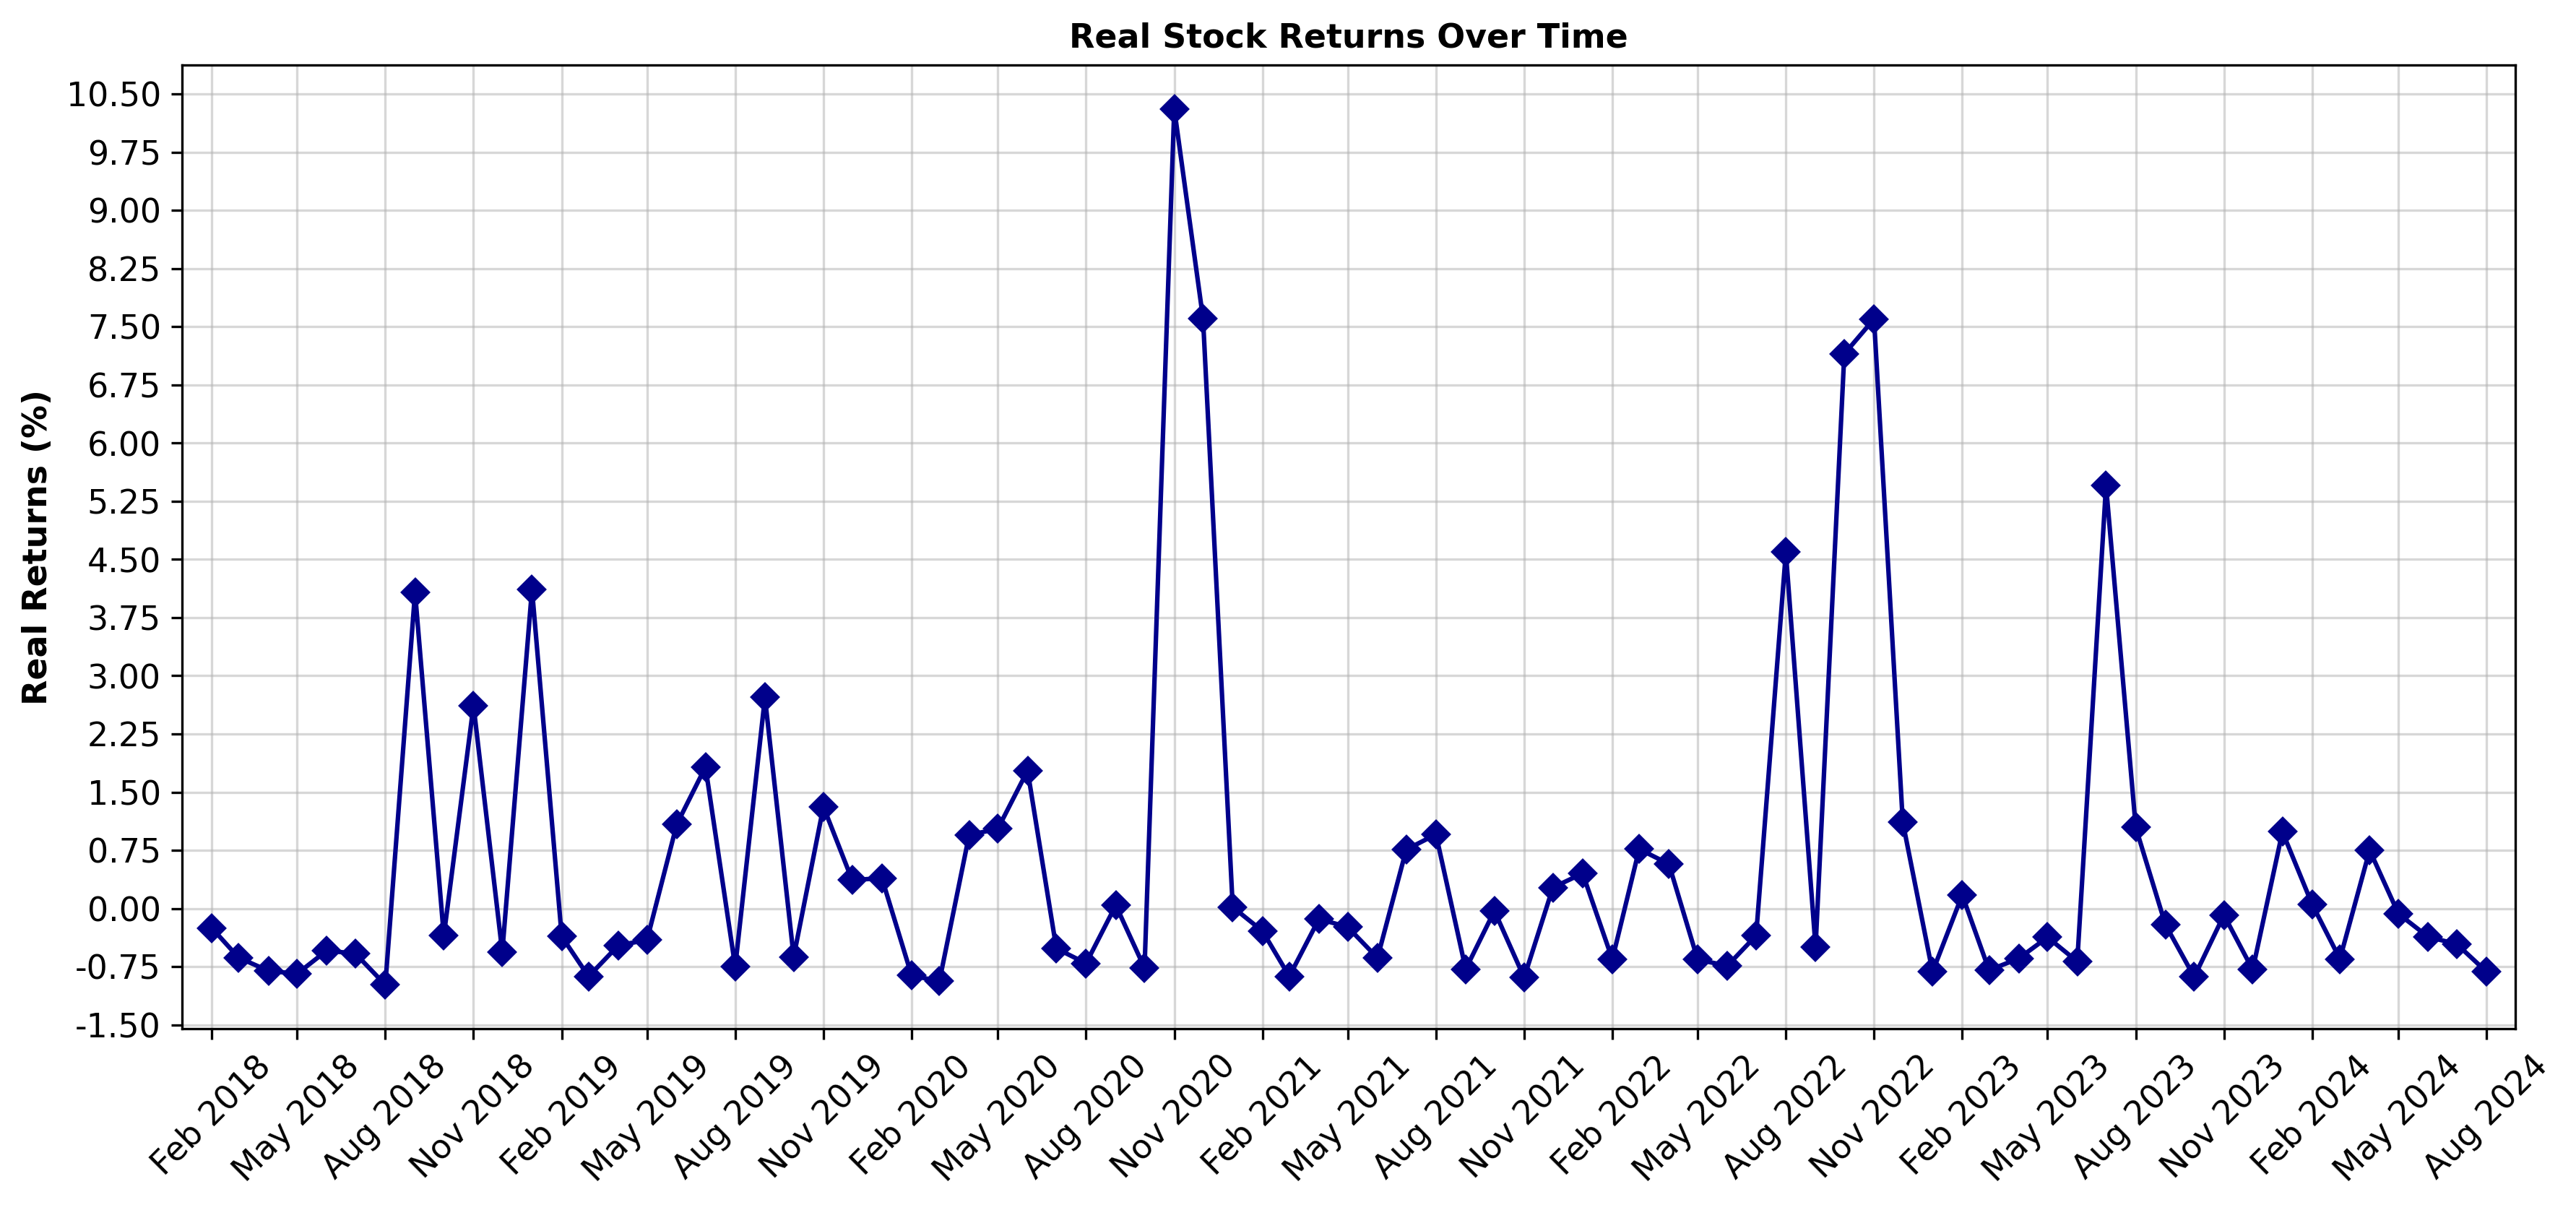
\includegraphics[width=0.7\textwidth]{real_stock_returns.png}
\begin{itemize}
\item Turkish stocks are highly volatile with several sharp peaks and periods of low or negative returns.
\item Turkish equities appear to offer opportunities for inflation hedging during certain periods, but are inconsistent as a hedge.
\item Stocks may reflect market optimism during inflationary periods, they still carry significant risks.
\end{itemize}
\end{frame}

\begin{frame}{Results: Turkish Government Bond}
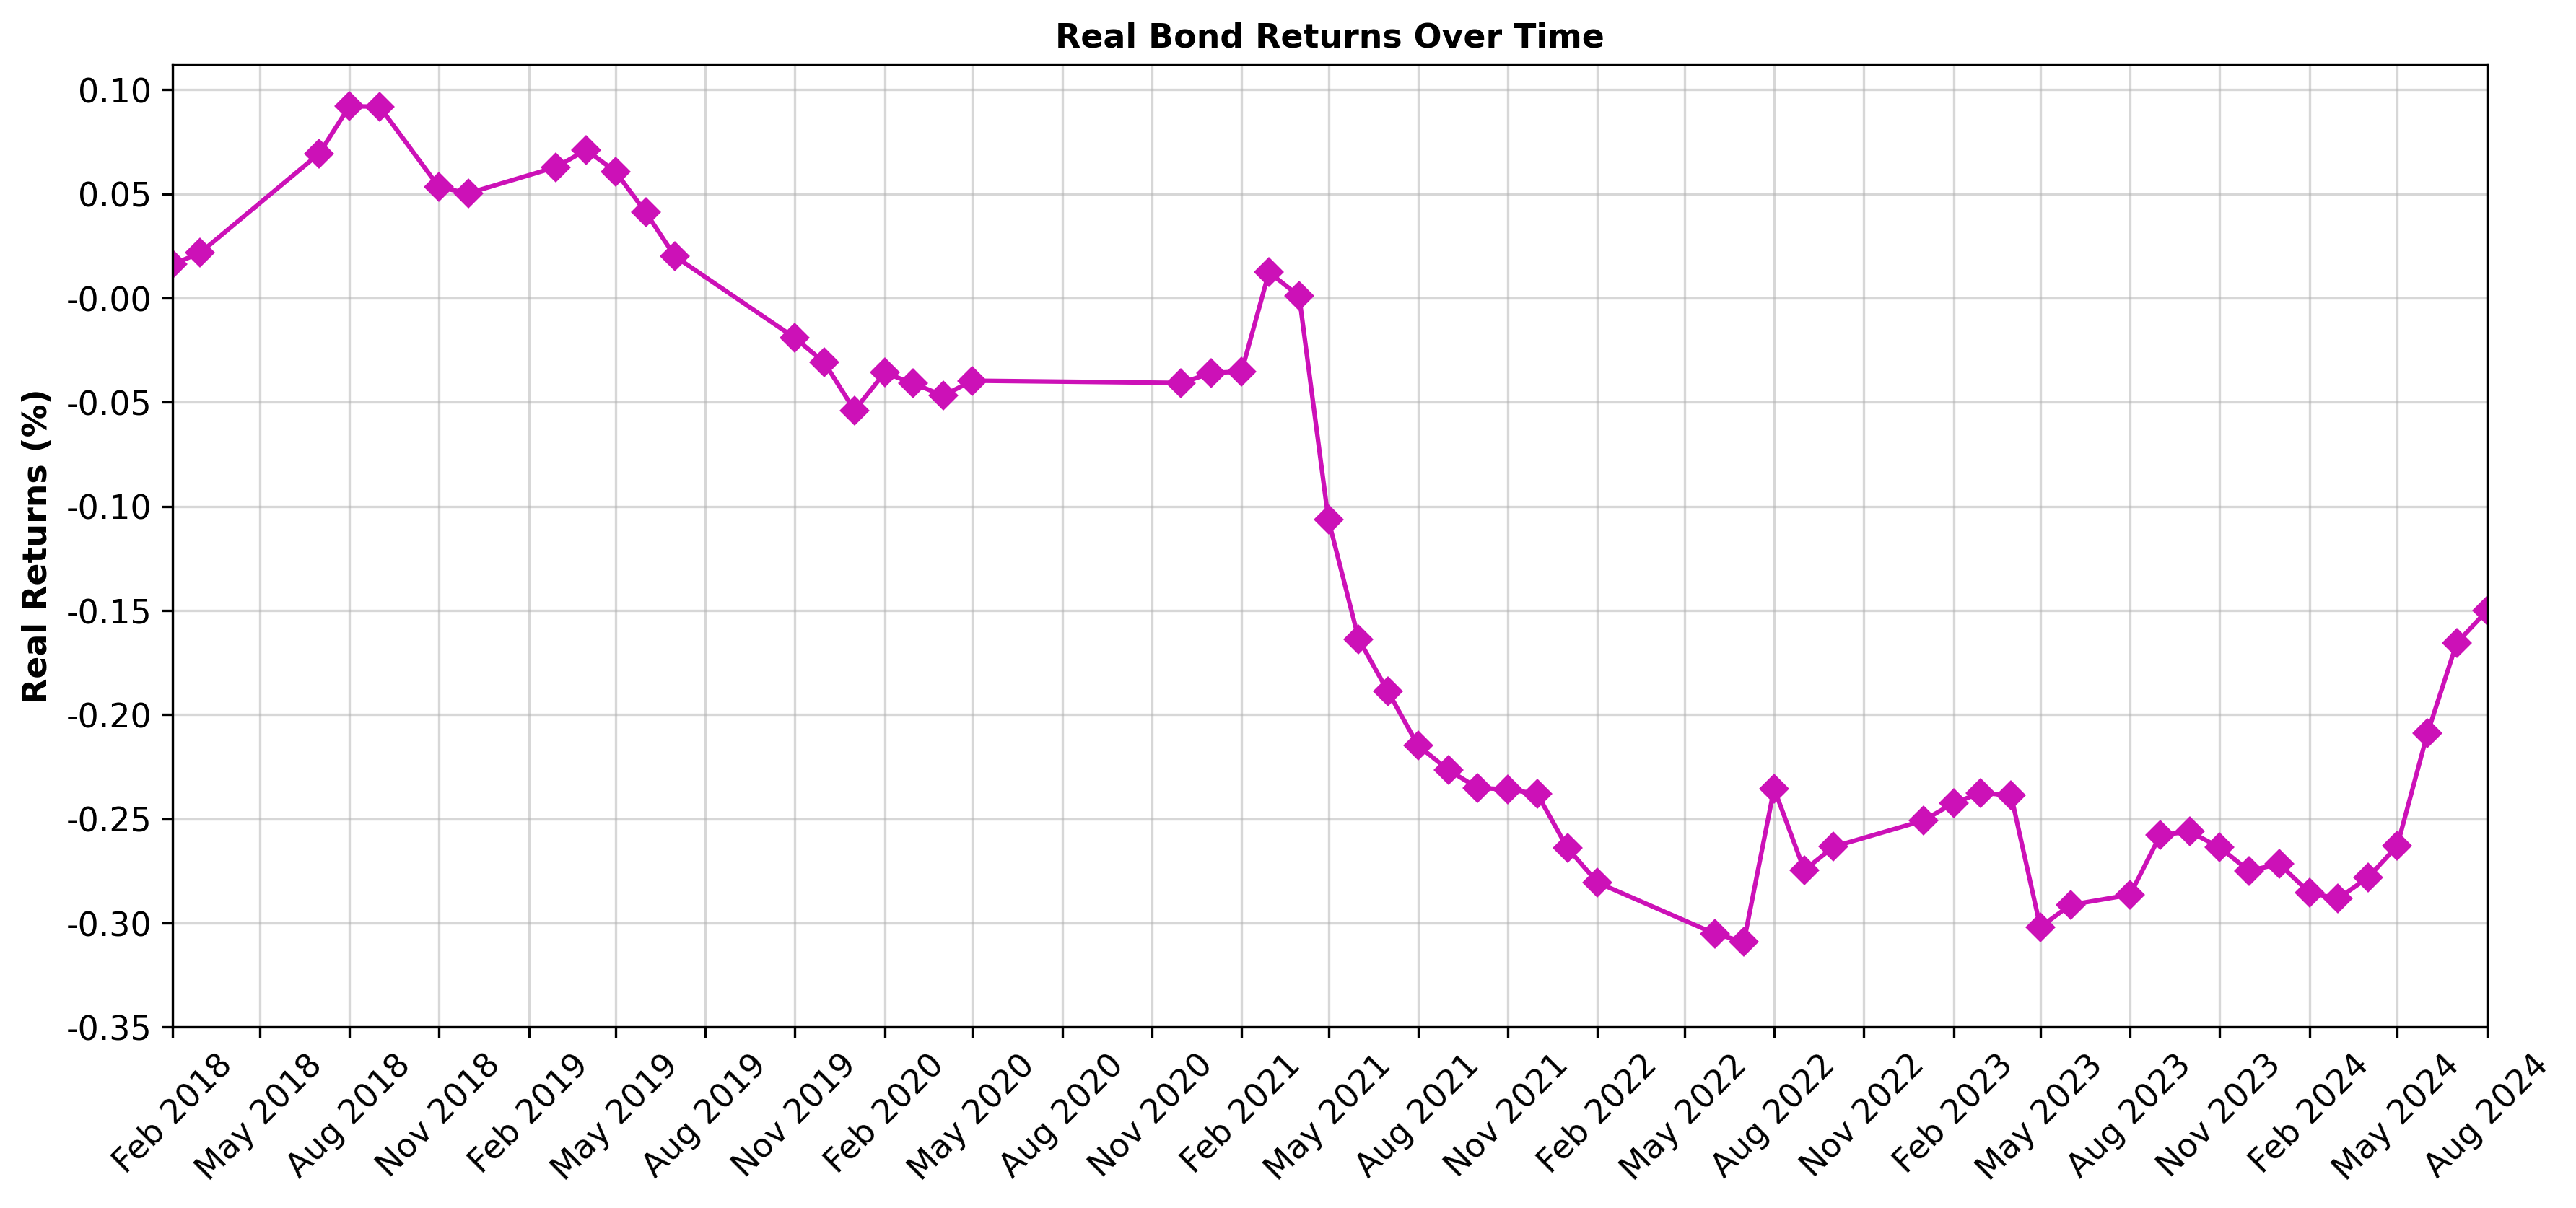
\includegraphics[width=0.7\textwidth]{real_bond_returns.png}
\begin{itemize}
\item Prolonged periods of negative real returns, especially as inflation rises.
\item Recent improvements in real returns may reflect monetary tightening, overall trend suggests that Turkish government bonds struggle to keep up with inflation.
\item Turkish bonds are not a good hedge against inflation due to their sensitivity to high inflation and credit risk.
\end{itemize}
\end{frame}

\begin{frame}{Results: Gold}
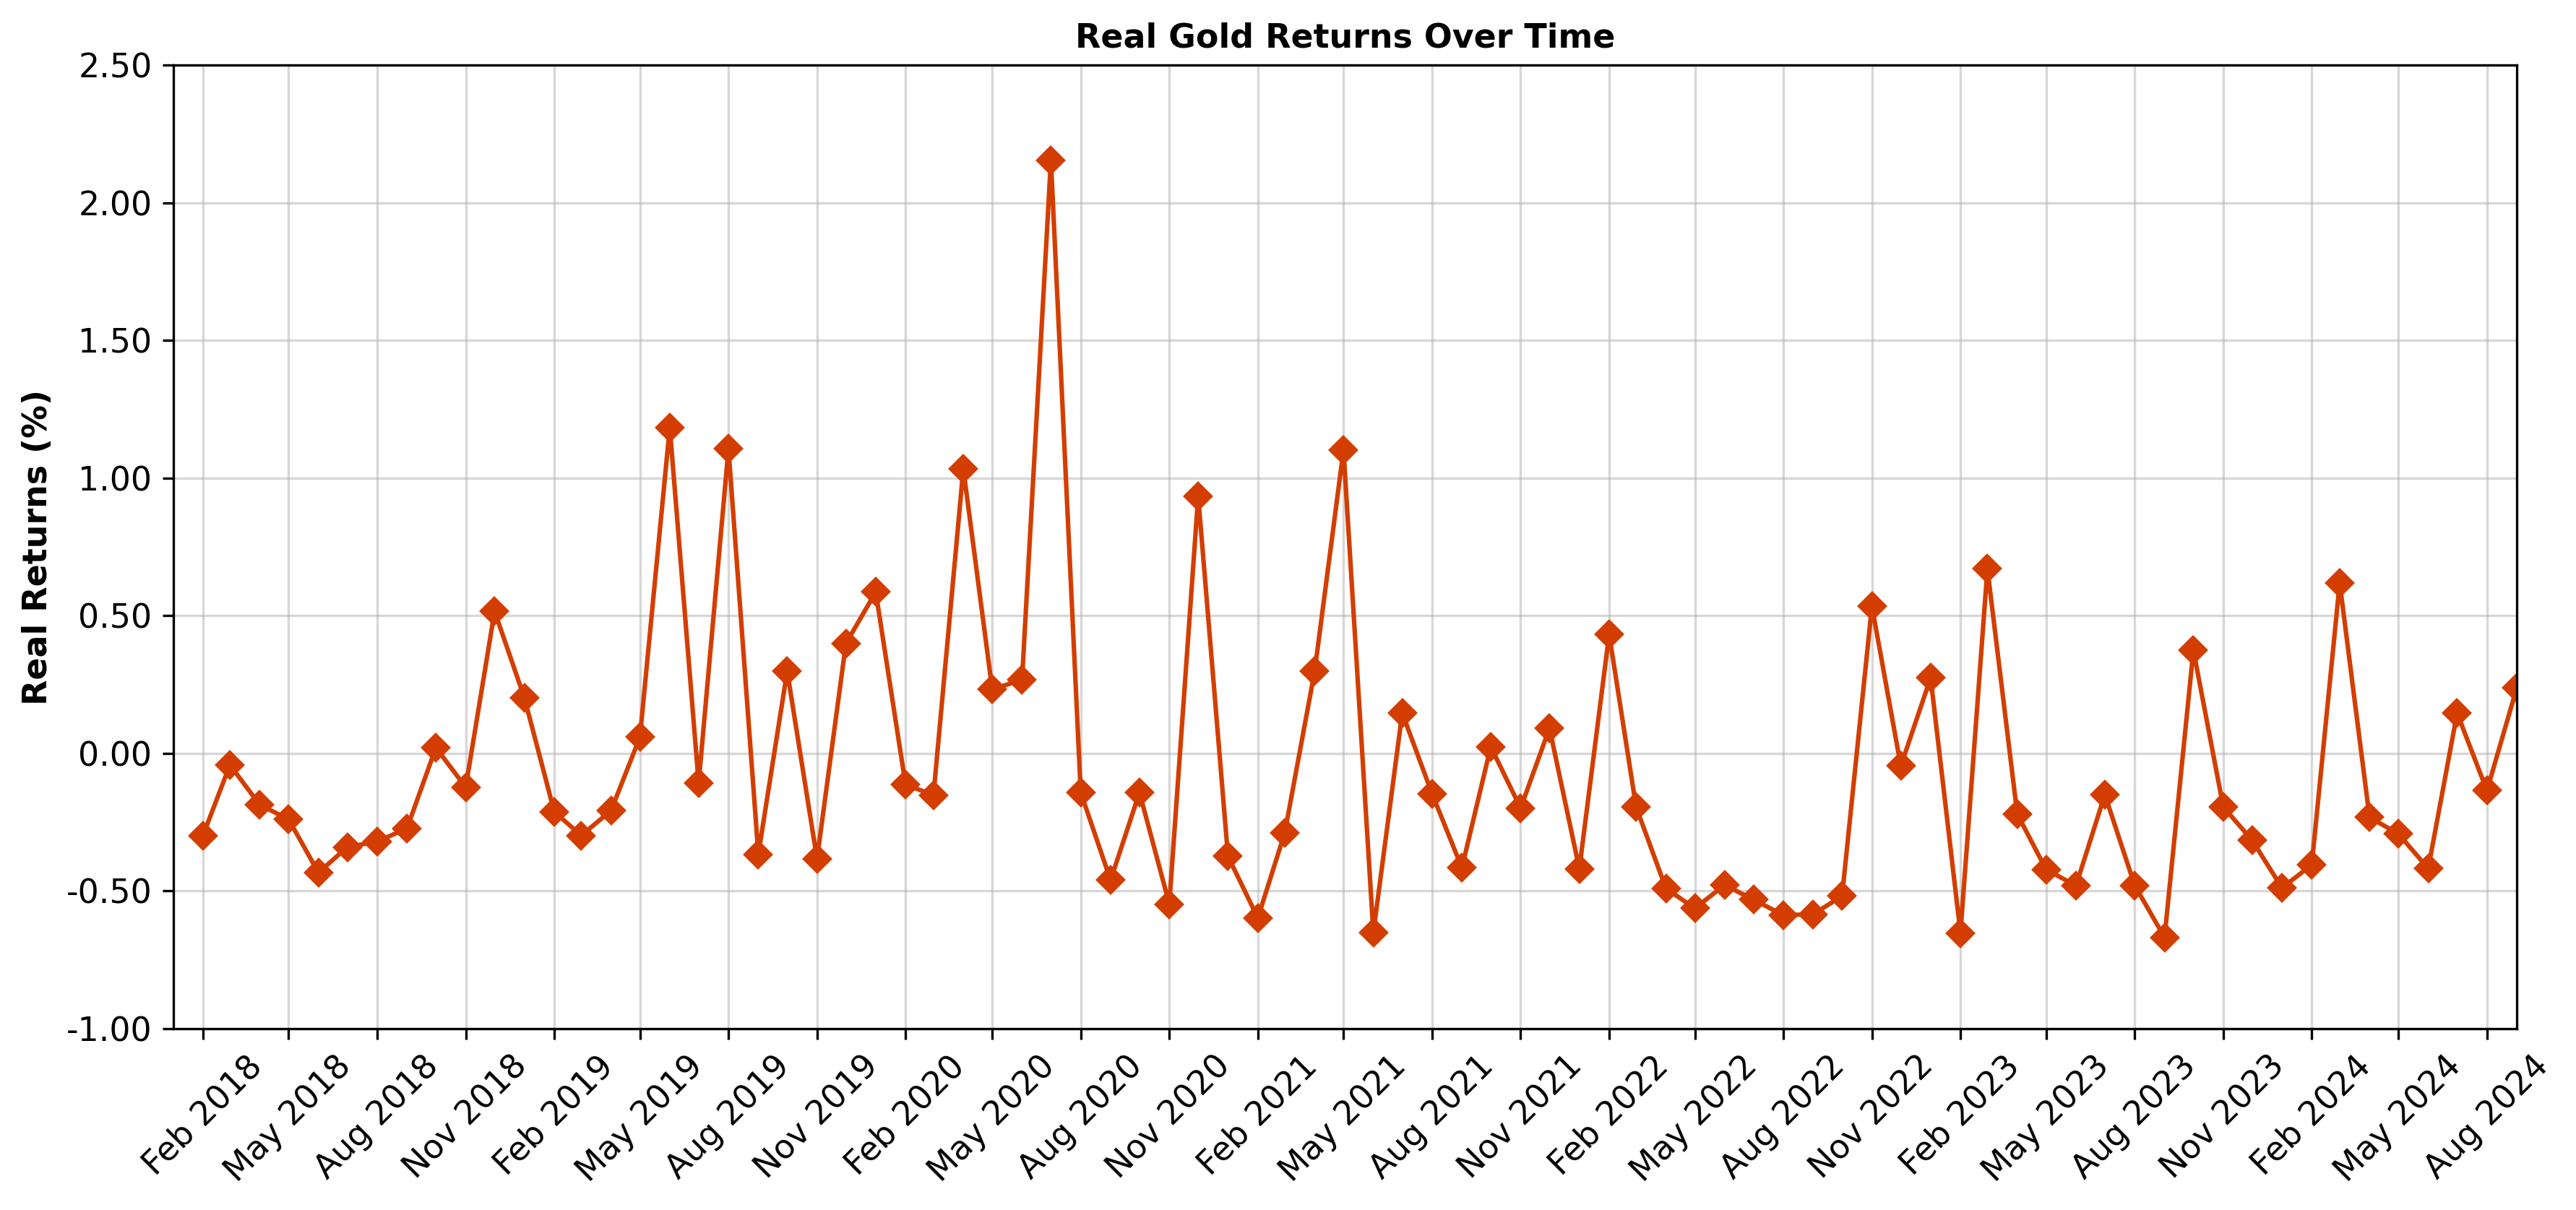
\includegraphics[width=0.7\textwidth]{real_gold_returns.png}
\begin{itemize}
\item Despite some negative returns, gold maintains a conistent performance compared to other assets.
\item This makes gold is a modest hedge against Turkish inflation, as it tends to hold its value during inflationary spikes. 
\end{itemize}
\end{frame}

\begin{frame}{Results: Bitcoin}
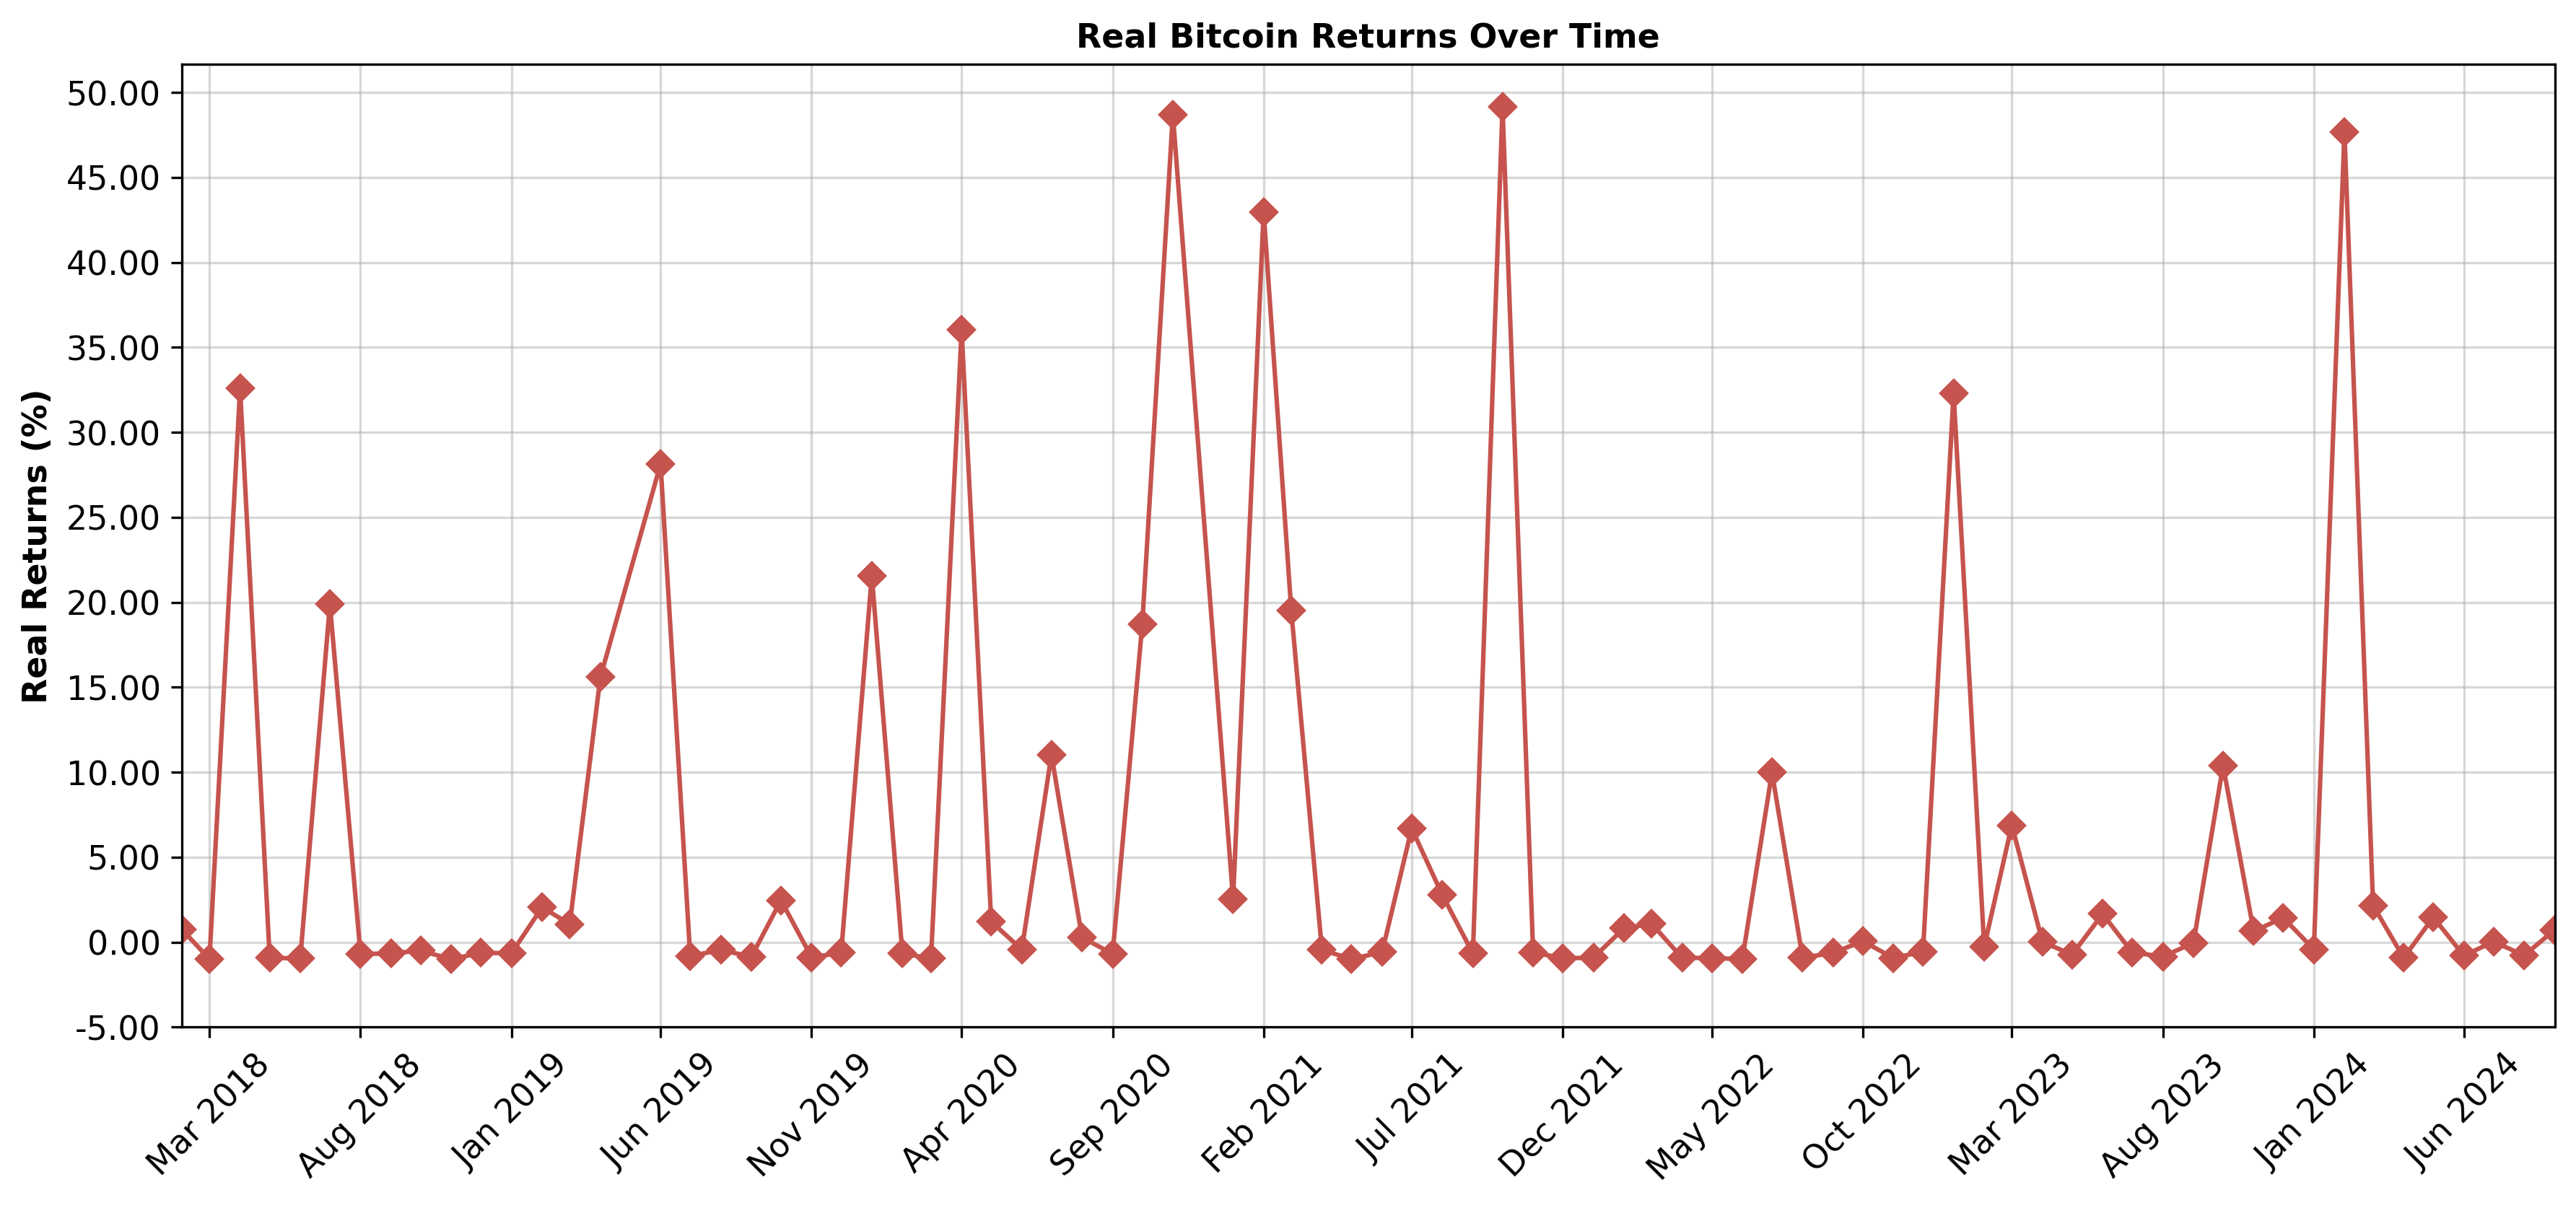
\includegraphics[width=0.7\textwidth]{real_bitcoin_returns.png}
\begin{itemize}
\item Bitcoin's real returns are highly volatile.
\item It occasionally generates high positive real returns but also shows frequent periods of near-zero or negative returns.
\item It is not a consistent hedge against Turkish inflation due to its high volatility. While it offers occasional large positive returns, it also carries significant downside risk.
\item sThis makes it speculative rather than a stable store of value in the context of inflation hedging.
\end{itemize}
\end{frame}

\begin{frame}{Results: Turkish Real Estate}
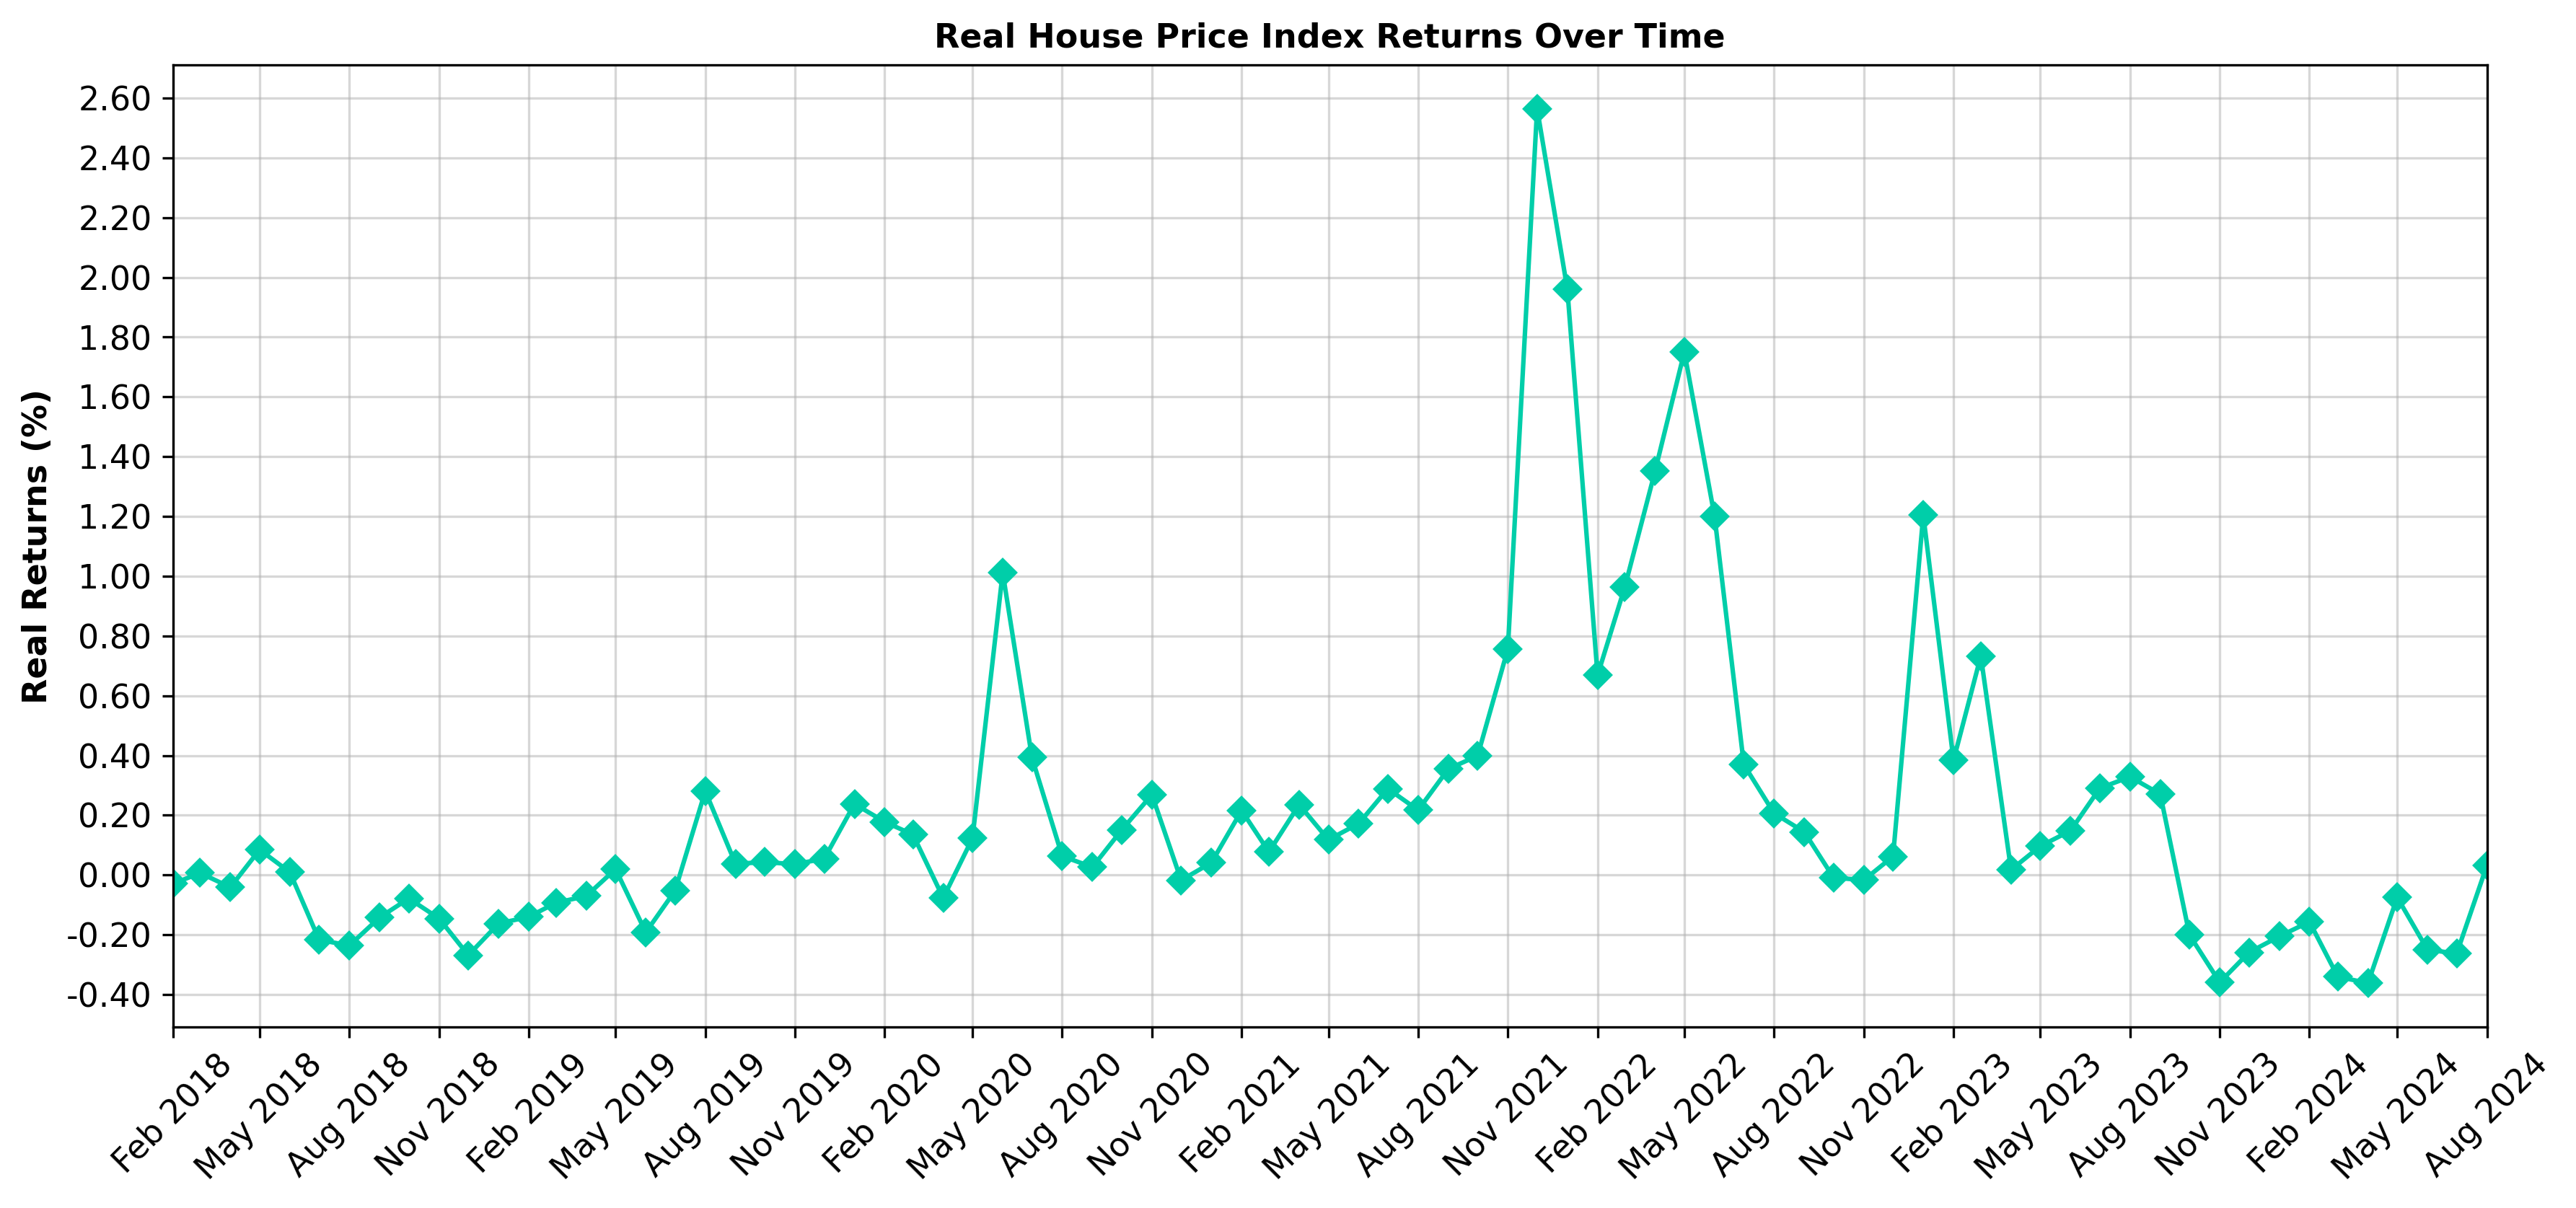
\includegraphics[width=0.7\textwidth]{real_hpi_returns.png}
\begin{itemize}
\item Real returns on Turkish real estate show occasional spikes, with also a few periods of slightly negative returns.
\item The peak in real returns occurred in late 2021, likely driven by a spike in inflation, with real estate acting as a safe haven.
\item Real estate appears to be a viable hedge against inflation during periods of high inflation in Türkiye. The sharp increase in real returns suggests strong investor demand for real assets to preserve wealth amid economic uncertainty.
\end{itemize}
\end{frame}

% Results: Markowitz Optimization
\begin{frame}{Results: Markowitz Optimization (mean risk-free)}
\begin{itemize}
    \item Portfolio allocation using the mean real return of the US 10y Gov Bond (-20.87\%):
    \begin{itemize}
        \item \textbf{Turkish Stocks:} 3.48\%
        \item \textbf{Turkish Government Bond:} 57.76\%
        \item \textbf{Gold:} 8.40\%
        \item \textbf{Bitcoin:} 0.15\%
        \item \textbf{Turkish Real Estate:} 30.21\%
    \end{itemize}
    \item Resulting in:
    \begin{itemize}
        \item \textbf{Expected Portfolio Return:} 1.34\%
        \item \textbf{Expected Portfolio Volatility:} 19.77\%
    \end{itemize}
\end{itemize}
\end{frame}

\begin{frame}{Results: Markowitz Optimization (median risk-free)}
\begin{itemize}
    \item Portfolio allocation using the median real return of the US 10y Gov Bond (-13.71\%):
    \begin{itemize}
        \item \textbf{Turkish Stocks:} 7.71\%
        \item \textbf{Turkish Government Bond:} 0.00\%
        \item \textbf{Gold:} 24.67\%
        \item \textbf{Bitcoin:} 0.47\%
        \item \textbf{Turkish Real Estate:} 67.15\%
    \end{itemize}
    \item Resulting in:
    \begin{itemize}
        \item \textbf{Expected Portfolio Return:} 22.05\%
        \item \textbf{Expected Portfolio Volatility:} 41.25\%
    \end{itemize}
\end{itemize}
\end{frame}

% Results: Markowitz Optimization
\begin{frame}{Results: Markowitz Optimization Interpretation}
\begin{itemize}
\item Portfolio allocation is highly sensitive to the choice of risk-free rate, highlighting the need for robust assumptions.
\item Using the mean real return (-20.87\%), the portfolio heavily allocates to Turkish government bonds (57.76\%) and real estate (30.21\%), with minimal allocation to gold (8.40\%) and bitcoin (0.15\%), targeting low risk (19.77\% volatility) and modest return (1.34\%).
\item Using the median real return (-13.71\%), allocations shift entirely to gold (24.67\%) and real estate (67.15\%), achieving a higher return (22.05\%) but with greater risk (41.25\% volatility).
\item Mean risk-free rate, sensitive to extreme values, results in conservative allocations with lower risk and returns.
\item Median risk-free rate, robust to outliers, drives aggressive allocations favoring higher returns at higher risk.
\item Markowitz optimization is mathematical, excluding behavioral factors and practical constraints like liquidity needs or volatility aversion.
\end{itemize}
\end{frame}

% Conclusion
\section{Conclusion and Future Research}
\begin{frame}{Conclusion}
\begin{itemize}
\item This study highlights the sensitivity of portfolio allocation to the choice of the real risk-free rate in inflation-adjusted Markowitz optimization.
\item Turkish real estate emerges as a key component in the portfolio, driven by its relatively high real returns and alignment with inflationary trends.
\item The resulting portfolio achieves high expected returns but is accompanied by significant volatility, particularly when the median real risk-free rate is used.
\end{itemize}
\end{frame}

\begin{frame}{Future Research}
\begin{itemize}
\item Future research could look into areas such as: 
\begin{itemize}
  \item Expand the asset universe to include more complex financial products, such as derivatives (e.g., inflation-linked swaps or options), exchange-traded funds (ETFs), or foreign-denominated assets. These products could provide more effective and flexible hedging mechanisms against inflation.
  \item Explore dynamic portfolio strategies that adapt to changing inflationary environments.
  \item Assess the role of alternative risk measures, such as downside risk or drawdown, to create portfolios that better address practical investor concerns.
\end{itemize}
\end{itemize}
\end{frame}

% Resources
\section{References}
\begin{frame}[allowframebreaks]{References}
\bibliography{references} % Ensure references.bib is in the same directory or update the path.
\end{frame}

\end{document}


